\documentclass[12pt]{extarticle}

\usepackage{geometry}
\usepackage{amsthm}
\usepackage{amssymb}
\usepackage{amsmath}
\usepackage{graphicx}

\graphicspath{ {./images/} }

\geometry{a4paper,
 total={170mm,257mm},
 left=20mm,
 top=20mm}

\title{Supervised Deep Learning for Optimized Trade Execution}
\author{Hua Wanying, Long Zijie, Wang Kunzhen}

\begin{document}
\maketitle

\section{Introduction}

\section{Literature Review}

\section{Model}
In this project, we assume that the optimal execution strategy can be expressed as
a pure function of the following 6 variables: $t$ the remaining time before the end of
the time horizon, $i$ the remaining inventory to sell, the price level, price trend,
limit order book volume mismatch as well as the bid-ask spread at the decision point.
Following the convention in \cite{reinforcement}, we group the 6 input variables
into two categories, i.e., the \textbf{private variables} consisting of $t$ and $i$
that is specific to the Optimized Trade Execution problem, and the \textbf{market variables}
consisting of the rest of the four. Output of the model is represented by \textit{\textbf{action}},
the price at which to place a limit order.
The model can be expressed mathematically as
$$ \textit{action} = f(t, i, \textit{price level}, \textit{price trend}, \textit{vol mismatch}, \textit{bid-ask spread}), $$
where $f$ is an unknown function to be learned. \\


\noindent To estimate the function $f$, we develop a supervised deep learning model as described below.
The model is implemented with \textit{Tensorflow} and \textit{Tensorflow
Keras} provided by Google Brain, using \textit{Python}.
Implementation of the model can be found in the file \textit{Model.py}.\\


\begin{figure}[h]
\centering
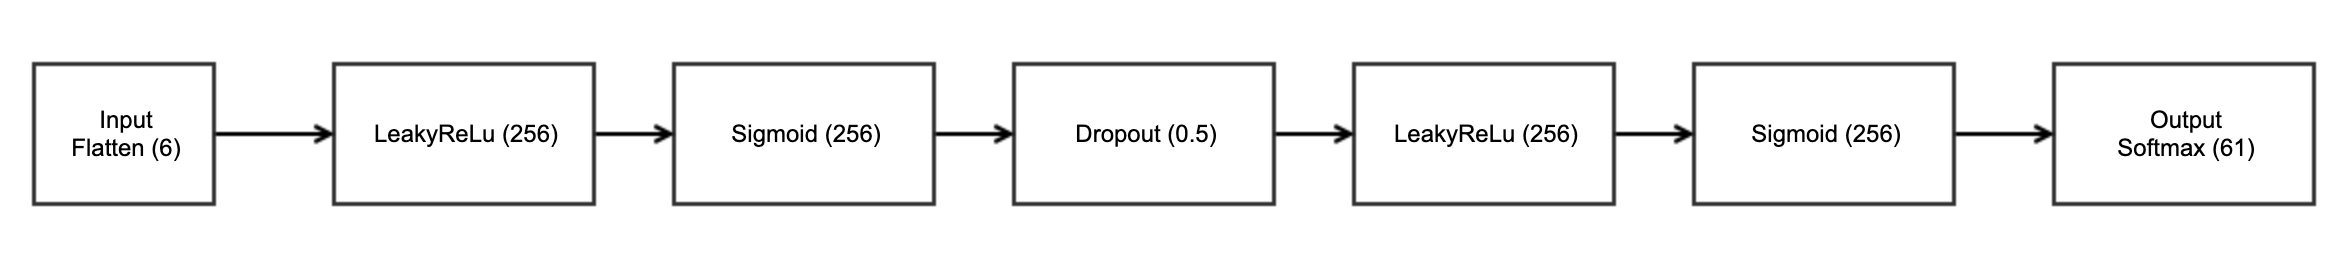
\includegraphics[width=\textwidth]{model}
\caption{The Supervised Deep Learning Model}
\end{figure}

\begin{itemize}
\item \textbf{Input Layer} The input layer consists of simply the 6 parameters of the function $f$.
Detailed definitions, rationales and extractions of these variables are
provided in Section \ref{market-variables} and \ref{private-variables}.

\item \textbf{Hidden Layers} The model is composed of 5 fully-connected hidden layers with
256 neurons each. Activation functions for each layer is, correspondingly,
\textit{leakyReLu},
\textit{sigmoid}, \textit{dropout} with a rate of 0.5,
\textit{leakyReLu}, \textit{sigmoid}. These activations are
chosen after taking into consideration the nature of the
problems. For example, noting the sparse activation characteristic of
the \textit{leakyReLu} activation and that the outputs are discrete, we chose \textit{leakyReLu}
to denoise the training process. Another advantage of the \textit{leakyReLu}
is its computational efficiency and ability to avoid dead neurons.
The \textit{sigmoid} activation is chosen for its ability to capture
non-linear relationships. A \textit{Dropout} layer is chosen
in the middle to denoise and speed up the descent. \\

\item \textbf{Output Layer} The output layer represents the predicted action given
the input. The output variable, \textit{\textbf{action}}, is discrete for computational
efficiency. Moreover, having a discretized output is important to avoid overfitting.
Refer to Section \ref{private-variables} for details on how \textit{\textbf{action}}
is discretized.

\end{itemize}


\section{Data Preparation}
This section describes in depth the dataset our research bases on and
how we extract the six aforementioned model inputs from the dataset.

\subsection{Data Description}

Describe the dataset and how we split it into training set vs testing set.

\subsection{Market Variables} \label{market-variables}

Describe the following:
\begin{itemize}
  \item How market variables are extracted from the dataset. Please include the exact formula.
  \item Rational of why those market variables are chosen.
\end{itemize}

\subsection{Private Variables} \label{private-variables}

Describe the following:
\begin{itemize}
  \item How private variables are extracted from the dataset. Please include details on
  dynamic programming (esp. formula), execution simulation, variable discretization and considerations.
\end{itemize}

\section{Model Training}


\section{Results}


\section{Remarks}

\section{Conclusion}

\begin{thebibliography}{9}
\bibitem{reinforcement}
Yuriy Nevmyvaka, Yi Feng, Michael Kearns.
\textit{Reinforcement Learning for Optimized Trade Execution}.
Proceedings of the 23rd International Conference on Machine Learning, Pittsburgh, PA, 2006.
\end{thebibliography}

\end{document}
